% !TEX encoding = UTF-8 Unicode
\documentclass{beamer}

\usepackage{color}
\usepackage{fancyvrb}
\usepackage{gensymb}
\usepackage{hyperref}
\usepackage{textcomp}
\usepackage{tikz}

\usetikzlibrary{arrows,positioning,shapes,shapes.multipart} 
\tikzstyle{every picture}+=[remember picture]

\definecolor{mygreen}{rgb}{0.88,0.95,0.88}

\usetheme{Warsaw}

\title[Data Visualization with R - Ggplot2 tutorial]{Data Visualization with R \\ Ggplot2 tutorial}
\author{Ariane Ducellier}
\date{University of Washington - Fall 2023}

\begin{document}

	\begin{frame}
		\titlepage
	\end{frame}

	\begin{frame}
		\frametitle{What is ggplot2?}

		Ggplot2 is the graphics package from the tidyverse, a collection of R packages designed for data science. 

		\vspace{2em}

		There is a base graphics package in R, which is present in the default version of R.

		\vspace{2em}

		However, ggplot2 gives users a lot more flexibility and control over their visualizations.
		
	\end{frame}

	\begin{frame}
		\frametitle{Main concepts of ggplot2}

		Ggplot2 is based on layers:

		\vspace{2em}
		
		\begin{itemize}
		\setlength{\itemsep}{1em}
			\item A first layer to describe the dataset.
			\item Layers describing the objects representing the data (dots, lines, bars, etc.).
			\item Additional objects describing the graphic itself (coordinates, scales, fonts, etc.)
		\end{itemize}

	\end{frame}

	\begin{frame}[fragile]
		\frametitle{Example: Histograms}

		Built-in R graphics package:

		\vspace{2em}

		\begin{exampleblock}{}
		\begin{center}
		\begin{BVerbatim}
		hist(airquality$Temp)
		\end{BVerbatim}
		\end{center}
		\end{exampleblock}{}

		\vspace{2em}

		Quick plot using ggplot2:

		\vspace{2em}

		\begin{exampleblock}{}
		\begin{center}
		\begin{BVerbatim}
		qplot(airquality$Temp)
		\end{BVerbatim}
		\end{center}
		\end{exampleblock}{}

	\end{frame}

	\begin{frame}[fragile]
		\frametitle{Ggplot2 command structure}

		\begin{exampleblock}{}
		\begin{center}
		\begin{BVerbatim}
		ggplot(airquality, aes(x=Temp))
		\end{BVerbatim}
		\end{center}
		\end{exampleblock}{}

		\vspace{2em}

		\begin{center}
		This command does not plot anything.
		\end{center}

		\vspace{2em}

		\begin{tikzpicture}
			\node[align=center, draw, rectangle, fill=mygreen] (l1) {
				\begin{BVerbatim}
				ggplot
				\end{BVerbatim}
			};
			\node[right=0.5cm of l1] (l2) [align=center, draw, rectangle, fill=mygreen] {
				\begin{BVerbatim}
				(
				\end{BVerbatim}
			};
			\node[right=0.5cm of l2] (l3) [align=center, draw, rectangle, fill=mygreen] {
				\begin{BVerbatim}
				airquality
				\end{BVerbatim}
			};
			\node[right=0.5cm of l3] (l4) [align=center, draw, rectangle, fill=mygreen] {
				\begin{BVerbatim}
				, aes(
				\end{BVerbatim}
			};
			\node[right=0.5cm of l4] (l5) [align=center, draw, rectangle, fill=mygreen] {
				\begin{BVerbatim}
				x=Temp
				\end{BVerbatim}
			};
			\node[right=0.5cm of l5] (l6) [align=center, draw, rectangle, fill=mygreen] {
				\begin{BVerbatim}
				))
				\end{BVerbatim}
			};

			\node[below=1cm of l1] (l7) [align=center, draw, rectangle, fill=mygreen] {Initialize object};
			\node[below=1cm of l3] (l8) [align=center, draw, rectangle, fill=mygreen] {Define the dataset};
			\node[below=1cm of l5] (l9) [align=center, draw, rectangle, fill=mygreen] {Define the variables};

			\path[draw,->, line width=1pt] (l7.north) -- node[above=0.5cm,left] {} (l1.south);
			\path[draw,->, line width=1pt] (l8.north) -- node[below=0.5cm,left] {} (l3.south);
			\path[draw,->, line width=1pt] (l9.north) -- node[above=0.5cm,left] {} (l5.south);
		\end{tikzpicture}

	\end{frame}

	\begin{frame}[fragile]
		\frametitle{Ggplot2 command structure}

		We need to add a command to explain the kind of object that we want to plot:

		\vspace{2em}

		\begin{exampleblock}{}
		\begin{BVerbatim}
		ggplot(airquality, aes(x=Temp)) +
		geom_histogram()
		\end{BVerbatim}
		\end{exampleblock}{}
		
	\end{frame}

	\begin{frame}[fragile]
		\frametitle{Bar plots}

		We can use bar plots to visualize one categorical variable:

		\vspace{2em}

		\begin{exampleblock}{}
		\begin{BVerbatim}
		ggplot(df_desc, aes(x=Vancouver)) +
		geom_bar()
		\end{BVerbatim}
		\end{exampleblock}{}

		\vspace{2em}

		The height of the bar is proportional to the number of cases in each group.
		
	\end{frame}

	\begin{frame}[fragile]
		\frametitle{Bar plots}

		Or a combination of a categorical variable and a continuous variable:

		\vspace{2em}

		\begin{exampleblock}{}
		\begin{BVerbatim}
		ggplot(RetailSales, aes(x=Month, y=Sales)) + 
		geom_bar(stat="identity")
		\end{BVerbatim}
		\end{exampleblock}{}

		\vspace{2em}

		Using \verb|stat = "identity"| tells ggplot2 to sum the values for each group (Month) and plot bars proportional to the sums.
		
	\end{frame}

	\begin{frame}[fragile]
		\frametitle{Box plots}

		For each layer that we want to add on our plot, we add the corresponding object:

		\vspace{2em}

		\begin{exampleblock}{}
		\begin{BVerbatim}
		ggplot(df_hum, aes(x=month, y=Vancouver)) + 
		geom_boxplot()
		\end{BVerbatim}
		\end{exampleblock}{}
		
	\end{frame}

	\begin{frame}[fragile]
		\frametitle{Scatter plots and line plots}

		The relationship between two continuous variables can be visualize with a scatter plot or a line plot:

		\vspace{2em}

		\begin{exampleblock}{}
		\begin{BVerbatim}
		ggplot(df, aes(x=time, y=distance)) +
		geom_point()
		\end{BVerbatim}
		\end{exampleblock}{}

		\vspace{2em}

		\begin{exampleblock}{}
		\begin{BVerbatim}
		ggplot(df, aes(x=time, y=distance)) +
		geom_line()
		\end{BVerbatim}
		\end{exampleblock}{}
		
	\end{frame}

	\begin{frame}[fragile]
		\frametitle{Changing histogram defaults}

		Modify the number of bins:

		\vspace{2em}

		\begin{exampleblock}{}
		\begin{BVerbatim}
		ggplot(df_hum, aes(x=Vancouver)) + 
		geom_histogram(bins=15)
		\end{BVerbatim}
		\end{exampleblock}{}

		\vspace{2em}

		Modify the filling and the color:

		\vspace{2em}

		\begin{exampleblock}{}
		\begin{BVerbatim}
		ggplot(df_hum, aes(x=Vancouver)) + 
		geom_histogram(bins=15, fill="white", color=1)
		\end{BVerbatim}
		\end{exampleblock}{}
	\end{frame}

	\begin{frame}[fragile]
		\frametitle{Adding aesthetics to the plot}

		Add title and axis labels to the histogram:

		\vspace{2em}

		\begin{exampleblock}{}
		\begin{BVerbatim}
		ggplot(df_hum, aes(x=Vancouver)) + 
		geom_histogram(bins=15, fill="white", color=1) +
		ggtitle("Humidity for Vancouver city") +
		xlab("Humidity") +
		theme(axis.text.x=element_text(size=12),
		axis.text.y=element_text(size=12))
		\end{BVerbatim}
		\end{exampleblock}{}
		
	\end{frame}

	\begin{frame}[fragile]
		\frametitle{Adding aesthetics to the boxplot}

		Add labels to the box plot:

		\vspace{2em}

		\begin{exampleblock}{}
		\begin{BVerbatim}
		ggplot(df_hum, aes(x=month, y=Vancouver)) + 
		geom_boxplot(color=1, fill=3) + 
		ylab("Humidity") + 
		theme(axis.text.x=element_text(size=15),
		axis.text.y=element_text(size=15),
		axis.title.x=element_text(size=15, color=2),
		axis.title.y=element_text(size=15, color=2))
		\end{BVerbatim}
		\end{exampleblock}{}
		
	\end{frame}

	\begin{frame}[fragile]
		\frametitle{Layers}

		Each plot can be thought as a separate variable, and the sum of the variables will make the final plot. You can define:

		\vspace{2em}

		\begin{exampleblock}{}
		\begin{BVerbatim}
		p1 <- ggplot(df,
		      aes(x=Electricity_consumption_per_capita))
		p2 <- p1 + geom_histogram()
		p3 <- p1 + geom_histogram(bins=15)
		p4 <- p3 + xlab("Electricity consumption per capita")
		\end{BVerbatim}
		\end{exampleblock}{}

		\vspace{2em}

		and you can choose to plot \verb|p2|, \verb|p3|, or \verb|p4|.

	\end{frame}

	\begin{frame}[fragile]
		\frametitle{Scales}

		Scales \verb|scale_x_continuous| or \verb|scale_x_discrete| can be used to specify the axes. \verb|name|, \verb|limits|, \verb|breaks|, and \verb|labels| are the main parameters that can be adjusted.

		\vspace{2em}

		\begin{exampleblock}{}
		\begin{BVerbatim}
		p1 <- ggplot(df, aes(x=gdp_per_capita))
		p2 <- p1 + geom_histogram()
		p3 <- p2 + scale_x_continuous(
		           name« "GDP per capita »),
		           limits=c(0, 50000),
		           breaks=seq(0, 40000, 4000),
		           labels=c("0K", "4K", "8K", "12K", "16K",
		           "20K",  "24K", "28K", "32K", "36K", "40K"))
		\end{BVerbatim}
		\end{exampleblock}{}

	\end{frame}

	\begin{frame}[fragile]
		\frametitle{Polar coordinates}

		You can define the coordinates with \verb|coord_cartesian| or \verb|coord_polar|:

		\vspace{2em}

		\begin{exampleblock}{}
		\begin{BVerbatim}
		t <- seq(0, 360, by=15)
		r <- 2
		qplot(r, t) +
		coord_polar(theta="y") +
		scale_y_continuous(breaks=seq(0, 360, 30))
		\end{BVerbatim}
		\end{exampleblock}{}

	\end{frame}

	\begin{frame}[fragile]
		\frametitle{Facets}

		A Trellis display allows creating a plot for each group of a categorical variable:

		\vspace{2em}

		\begin{exampleblock}{}
		\begin{BVerbatim}
		p <- ggplot(df,
		     aes(x=gdp_per_capita,
		     y=Electricity_consumption_per_capita)) +
		     geom_point()
		p + facet_grid(Country ~ .)
		p + facet_grid(. ~ Country)
		p + facet_wrap(~Country)
		\end{BVerbatim}
		\end{exampleblock}{}

		\vspace{2em}

		You can group subplots horizontally, vertically or wrapped together.

	\end{frame}

	\begin{frame}[fragile]
		\frametitle{Shapes and colors}

		You can change shape and color for the entire plot:

		\vspace{2em}

		\begin{exampleblock}{}
		\begin{BVerbatim}
		ggplot(df, aes_string(x=var1, y=var2)) +
		geom_point(color=2, shape=2)
		\end{BVerbatim}
		\end{exampleblock}{}

		\vspace{2em}

		Or assign a different shape and color for each group of a categorical variable:

		\vspace{2em}

		\begin{exampleblock}{}
		\begin{BVerbatim}
		ggplot(df, aes_string(x=var1, y=var2)) +
		geom_point(aes(color=Country, shape=Country))
		\end{BVerbatim}
		\end{exampleblock}{}

	\end{frame}

	\begin{frame}[fragile]
		\frametitle{Themes}

		Theme is used to change the non-data elements of the plot:

		\vspace{1em}

		\begin{center}
		\begin{tabular}{|l|l|l|}
		\hline
    		Theme & Type & Arguments \\ 
		\hline
		axis.title.x & element\_text & size, color, family, angle \\
		\hline
		axis.title.y & element\_text & size, color, family, angle \\
		\hline
		plot.background & element\_rect & fill, color, linewidth \\
		\hline
		panel.background & element\_rect & fill, fill, color, line width \\
		\hline
		panel.grid.major & element\_line & color, linetype, linewidth \\
		\hline
		\end{tabular}
		\end{center}

		\vspace{1em}

		Type \verb|?theme| to show all possible types of themes, their types and their arguments.

	\end{frame}

	\begin{frame}[fragile]
		\frametitle{Themes}

		You can add themes to the plot to customize the non-data elements:

		\vspace{1em}

		\begin{exampleblock}{}
		\begin{BVerbatim}
		p1 <- ggplot(dfn, aes(Genre, WorldGross)) 
		p2 <- p1+ geom_bar(aes(fill=LeadStudio), 
		                       stat="Identity",
		                       position="dodge")
		p3 <- p2 + theme(axis.title.x=element_text(size=15),
		                 axis.title.y=element_text(size=15),
		plot.background=element_rect(fill="gray87"),
		panel.background=element_rect(fill="beige"),
		panel.grid.major=element_line(color="Gray",
		                              linetype=1))
		\end{BVerbatim}
		\end{exampleblock}{}

	\end{frame}

	\begin{frame}[fragile]
		\frametitle{Themes}

		You can use predefined themes:

		\vspace{2em}

		\begin{exampleblock}{}
		\begin{BVerbatim}
		p2 + theme_bw() + ggtitle("theme_bw()")
		p2 + theme_classic() + ggtitle("theme_classic()")
		p2 + theme_classic() + ggtitle("theme_gray()")
		p2 + theme_minimal() + ggtitle("theme_minimal()")
		\end{BVerbatim}
		\end{exampleblock}{}

	\end{frame}

	\begin{frame}[fragile]
		\frametitle{Themes}

		You can also use define your own theme:

		\begin{exampleblock}{}
		\begin{BVerbatim}
		mytheme <- theme(legend.title=element_blank(),
		legend.position="bottom",
		text=element_text(color="Blue"),
		axis.text=element_text(size=12, color="Red"),
		axis.title=element_text(size=rel(1.5)))
		\end{BVerbatim}
		\end{exampleblock}{}

		and use it for a single plot:

		\begin{exampleblock}{}
		\begin{BVerbatim}
		p2 + mytheme + ggtitle("Changed Plot with my theme")
		\end{BVerbatim}
		\end{exampleblock}{}

		or for all the plots by placing it at the beginning of your code:

		\begin{exampleblock}{}
		\begin{BVerbatim}
		theme_set(my_theme)
		\end{BVerbatim}
		\end{exampleblock}{}

	\end{frame}

	\begin{frame}[fragile]
		\frametitle{Themes}

		You can change the color palette.

		\vspace{2em}

		Type \verb|?scale_fill_brewer| to see all the color palettes available.

		\vspace{2em}

		\begin{exampleblock}{}
		\begin{BVerbatim}
		p4 <- p2 + theme_bw() + ggtitle("theme_bw()")
		p4 + scale_fill_brewer(palette="Spectral")
		\end{BVerbatim}
		\end{exampleblock}{}

	\end{frame}

	\begin{frame}[fragile]
		\frametitle{Bubble charts}

		You can make the size of each marker proportional to a variable:

		\vspace{2em}

		\begin{exampleblock}{}
		\begin{BVerbatim}
		ggplot(dfs, aes(x=Year,
		                y=Electricity_consumption_per_capita))
		+ geom_point(aes(size=population, color=Country))
		+ scale_size(breaks=c(0, 1e+8, 0.3e+9, 0.5e+9,
		                      1e+9, 1.5e+9), range=c(1, 5))
		\end{BVerbatim}
		\end{exampleblock}{}

	\end{frame}

	\begin{frame}[fragile]
		\frametitle{Density plots}

		Instead of plotting an histogram, ggplot2 will estimate the density before plotting it:

		\vspace{1em}

		\begin{exampleblock}{}
		\begin{BVerbatim}
		ggplot(df, aes(x=loan_amnt)) + 
		geom_density() + 
		facet_wrap(~grade)
		\end{BVerbatim}
		\end{exampleblock}{}

		\vspace{1em}

		It is also possible to superimpose the density plots:

		\vspace{1em}
	
		\begin{exampleblock}{}
		\begin{BVerbatim}
		ggplot(df, aes(x=loan_amnt)) + 
		geom_density(aes(fill=grade), alpha=1/2) +
		scale_fill_brewer(palette="Dark2")
		\end{BVerbatim}
		\end{exampleblock}{}

	\end{frame}

	\begin{frame}[fragile]
		\frametitle{Time series plots}

		Use\verb|geom_line| to make time series plots:

		\vspace{2em}

		\begin{exampleblock}{}
		\begin{BVerbatim}
		df_fb$Date <- as.Date(df_fb$Date)
		ggplot(df_fb, aes(x=Date, y=Close, group=1)) + 
		geom_line(color="black", na.rm=TRUE) +
		scale_x_date(date_breaks='3 month')
		\end{BVerbatim}
		\end{exampleblock}{}

		\vspace{2em}

		We use \verb|group=1| one there is only one line to be show.

		\vspace{2em}

		Use \verb|group=MyCategory| to plot a line per value of a categorical variable.

	\end{frame}

	\begin{frame}[fragile]
		\frametitle{Statistical summaries}

		You can add statistical summaries of the data (e.g. mean, median, quantiles) to the plot:

		\vspace{2em}
	
		\begin{exampleblock}{}
		\begin{BVerbatim}
		ggplot(df_fb, aes(Month, Close)) + 
		geom_point(color="red", alpha=1/2,
		           position=position_jitter(h=0.0, w=0.0)) +
		stat_summary(geom="line", fun="quantile",
		             fun.args=list(probs=.1), linetype=2,
		             color="green", size=1) +
		stat_summary(geom="line", fun="quantile",
		             fun.args=list(probs=.9), linetype=2,
		             color="green", size=1)
		\end{BVerbatim}
		\end{exampleblock}{}

	\end{frame}

	\begin{frame}[fragile]
		\frametitle{Linear regression}

		Ggplot can also fit a linear regression to the data and add it to the plot. It may be done for all the data:

		\vspace{2em}
	
		\begin{exampleblock}{}
		\begin{BVerbatim}
		ggplot(dfs, aes(gdp_per_capita,
		                Electricity_consumption_per_capita)) +
		geom_point(aes(color=Country)) +
		stat_smooth(method=lm)
		\end{BVerbatim}
		\end{exampleblock}{}

	\end{frame}

	\begin{frame}[fragile]
		\frametitle{Linear regression}

		Or you can fit a linear regression to each category:

		\vspace{2em}
	
		\begin{exampleblock}{}
		\begin{BVerbatim}
		ggplot(dfs, aes(gdp_per_capita,
		                 Electricity_consumption_per_capita,
		                 color=Country)) +
		geom_point() +
		stat_smooth(method=lm)
		\end{BVerbatim}
		\end{exampleblock}{}

	\end{frame}

	\begin{frame}[fragile]
		\frametitle{Correlations}

		You can also plot correlations between different variables:

		\vspace{2em}
	
		\begin{exampleblock}{}
		\begin{BVerbatim}
		M <- cor(df)
		corrplot(M, method="number")
		corrplot(M, method="pie")
		corrplot(M, method="ellipse")
		\end{BVerbatim}
		\end{exampleblock}{}

	\end{frame}

	\begin{frame}[fragile]
		\frametitle{Maps}

		You can use maps from the \verb|maps| and \verb|map_data| packages to plot maps:

		\vspace{1em}
	
		\begin{exampleblock}{}
		\begin{BVerbatim}
		world_map <- map_data("world")
		states_map <- map_data("state")
		\end{BVerbatim}
		\end{exampleblock}{}

		\vspace{1em}

		You can select only some polygons from the map using:

		\vspace{1em}

		\begin{exampleblock}{}
		\begin{BVerbatim}
		europe <- map_data("world",
		region=c("Germany", "Spain", "Italy",
		         "France", "UK", "Ireland")) 
		\end{BVerbatim}
		\end{exampleblock}{}

	\end{frame}

	\begin{frame}[fragile]
		\frametitle{Maps}

		To plot the data, we may use \verb|geom_polygom| or \verb|geom_path|.

		\vspace{2em}

		The projection is defined with \verb|coord_map|.

		\vspace{2em}
	
		\begin{exampleblock}{}
		\begin{BVerbatim}
		ggplot(states_map, aes(x=long, y=lat, group=group)) +
		geom_polygon(fill="white", color="black")
		\end{BVerbatim}
		\end{exampleblock}{}

		\vspace{2em}

		\begin{exampleblock}{}
		\begin{BVerbatim}
		ggplot(states_map, aes(x=long, y=lat, group=group)) +
		geom_path() +
		coord_map("mercator")
		\end{BVerbatim}
		\end{exampleblock}{}

	\end{frame}

\end{document}
